\section{ICD コンプライアンス}

本衛星は,イプシロンロケット4号機での打ち上げにあたり,そのインターフェー
ス仕様がJX-ESPC-101655 インターフェース管理文書 OrigamiSat-1\/イプシロ
ンロケット4号機により定められている.安全審査と並行して,本インターフェー
ス管理文書(Interface Control Document, ICD)への適合についての確認が
進められた.ICD適合については,OP-S1-0127 OrigamiSat-1 ICDコンプライア
ンスマトリクス にて管理を行った.適合結果の詳細については,同文書の記
載およびエビデンス文書情報については,同文書を参照されたい.

\section{ICD 適合に関して生じた問題}

本衛星の衛星FM製作にあたり,ICD 適合に対して以下の問題が生じたが,対処
の結果全て適合となった.

\subsection{レールの長さ}
本ICDでは衛星放出ポッド (E-SSOD) と接するレール部について,「 各レール
  の±Zを除く側面について、E-SSODのガイドレールと少なくとも 75\% 以上、上
  述の規定に基づく接触面をもつこと。(すなわち、レールの接触面として、3Uの場合
    255.4mm以上を有すること。)」という規定があり,本衛星はレール長さ
が 75.3\% となる設計としていた.しかし,一部にレールと衛星構体を固定するためのネジ穴お
よび座繰り部分が存在したため,この部分をレール部から除外されることとなっ
た結果,レール長さが 67.1\% となり,ICD逸脱となってしまった.

ロケット側との協議の結果,試験用 E-SSODを用いて出動作時の動摩擦の計測および引抜
試験を実施し,同試験について実用上問題無いことが確認された
ため上記設計のままで良いこととなった.

本件は,「レール」の定義について認識に齟齬があったことに起因している.
インターフェースに関わる部分・部品については,名前の定義を十分にすり合
わせることが肝要である.

\subsection{ポッド側レール端部の切り欠き処理に伴う接触面不足}
E-SSODとのフィットチェックにおいて,E-SSODのレールは放出口側の端部が開
く形でICDに記載のない切り欠きがついていることが判明した.一方で,本衛
星は膜展開部のレールは膜展開動作を阻害しないように大きくレールの無い区間を大きく
とってあり,衛星先端部のレールは 1cm 程度の長さとなっていた.本衛星で
は,膜展開部側を放出方向と規定していたため,衛星端部の短いレール部
分が上記の切り欠き部の位置に相当することとなり,衛星端部から膜展開部根
本までの区間が固定されない片持ち梁の状態となってしまうことが判明した.

対応として,衛星の放出方向を逆とすることにより,十分にレール長さのある部分が
切り欠き部の位置に来るようにした.但しこれに伴い,放出検知スイッチの動作を
防止し,E-SSODの放出扉を閉め放出検知スイッチが常時押下状態となった後に
取り外す予定だった2つのフライトピンがE-SSODのアクセス窓(放出扉を閉めた後にフラ
  イトピンを抜くための窓)の反対側に位置することとなり,衛星収納後にア
クセスできなくなってしまった.そのため,衛星収納作業時に放出検知スイッ
チをカプトンテープで固定し,E-SSODへの挿入を行う様,手法および手順を変
更することとなった.本事象の内容・対処の詳細について,図\ref{6_1_trouble2}に
示す.

\begin{figure}[htbp]
\centering
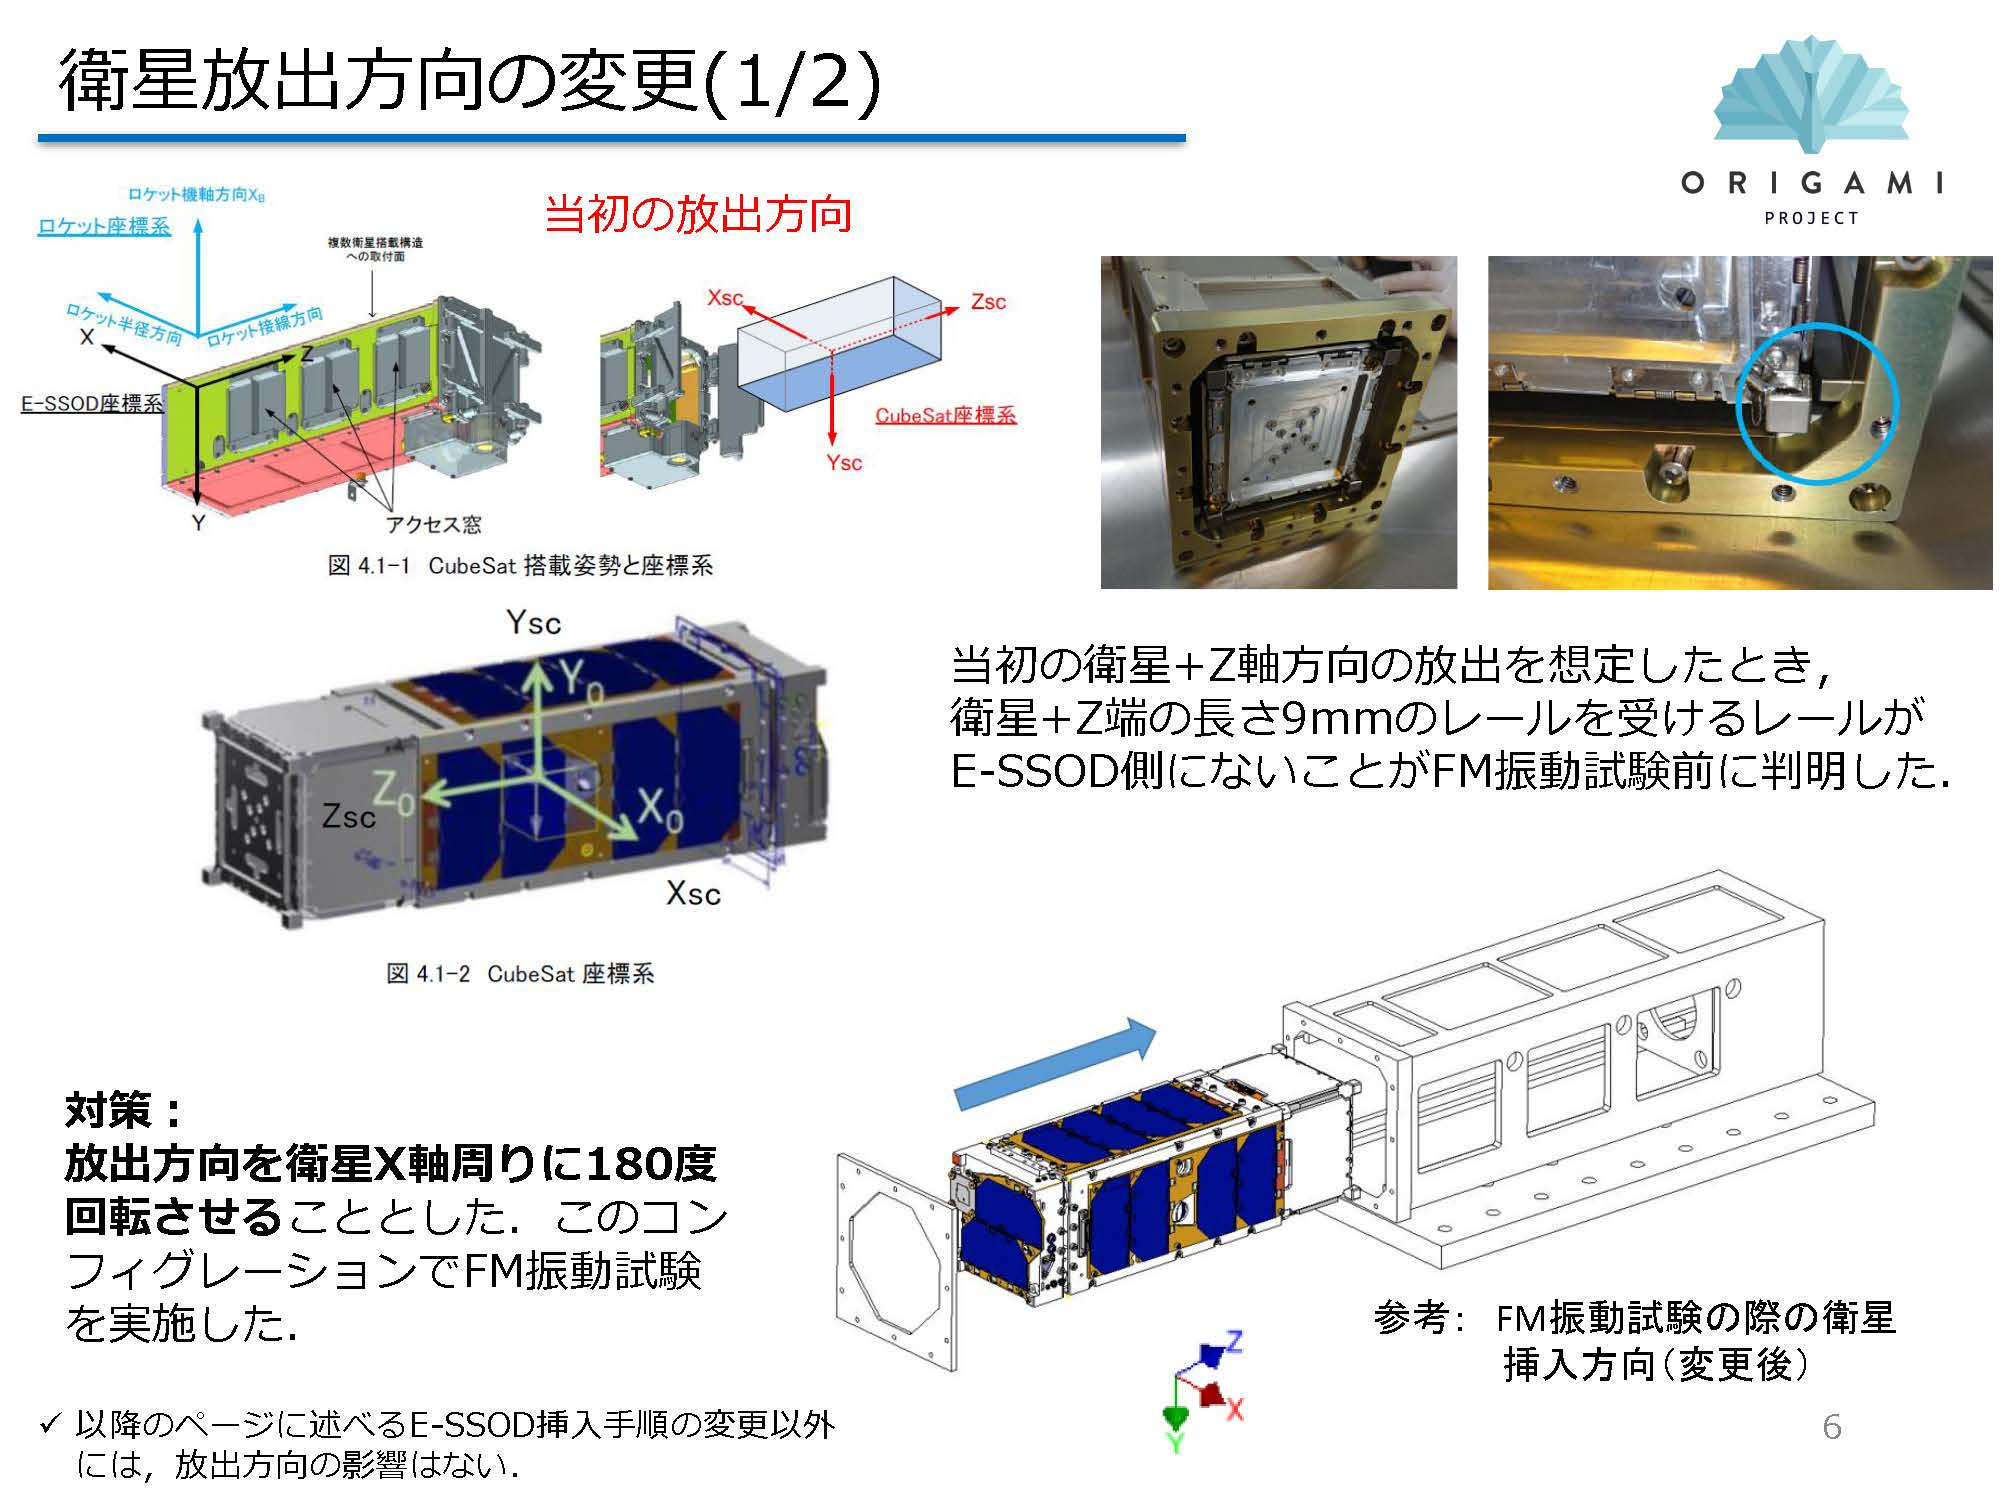
\includegraphics[width=10cm]{./06/fig/6-1_rail_trouble_2-1.jpg}
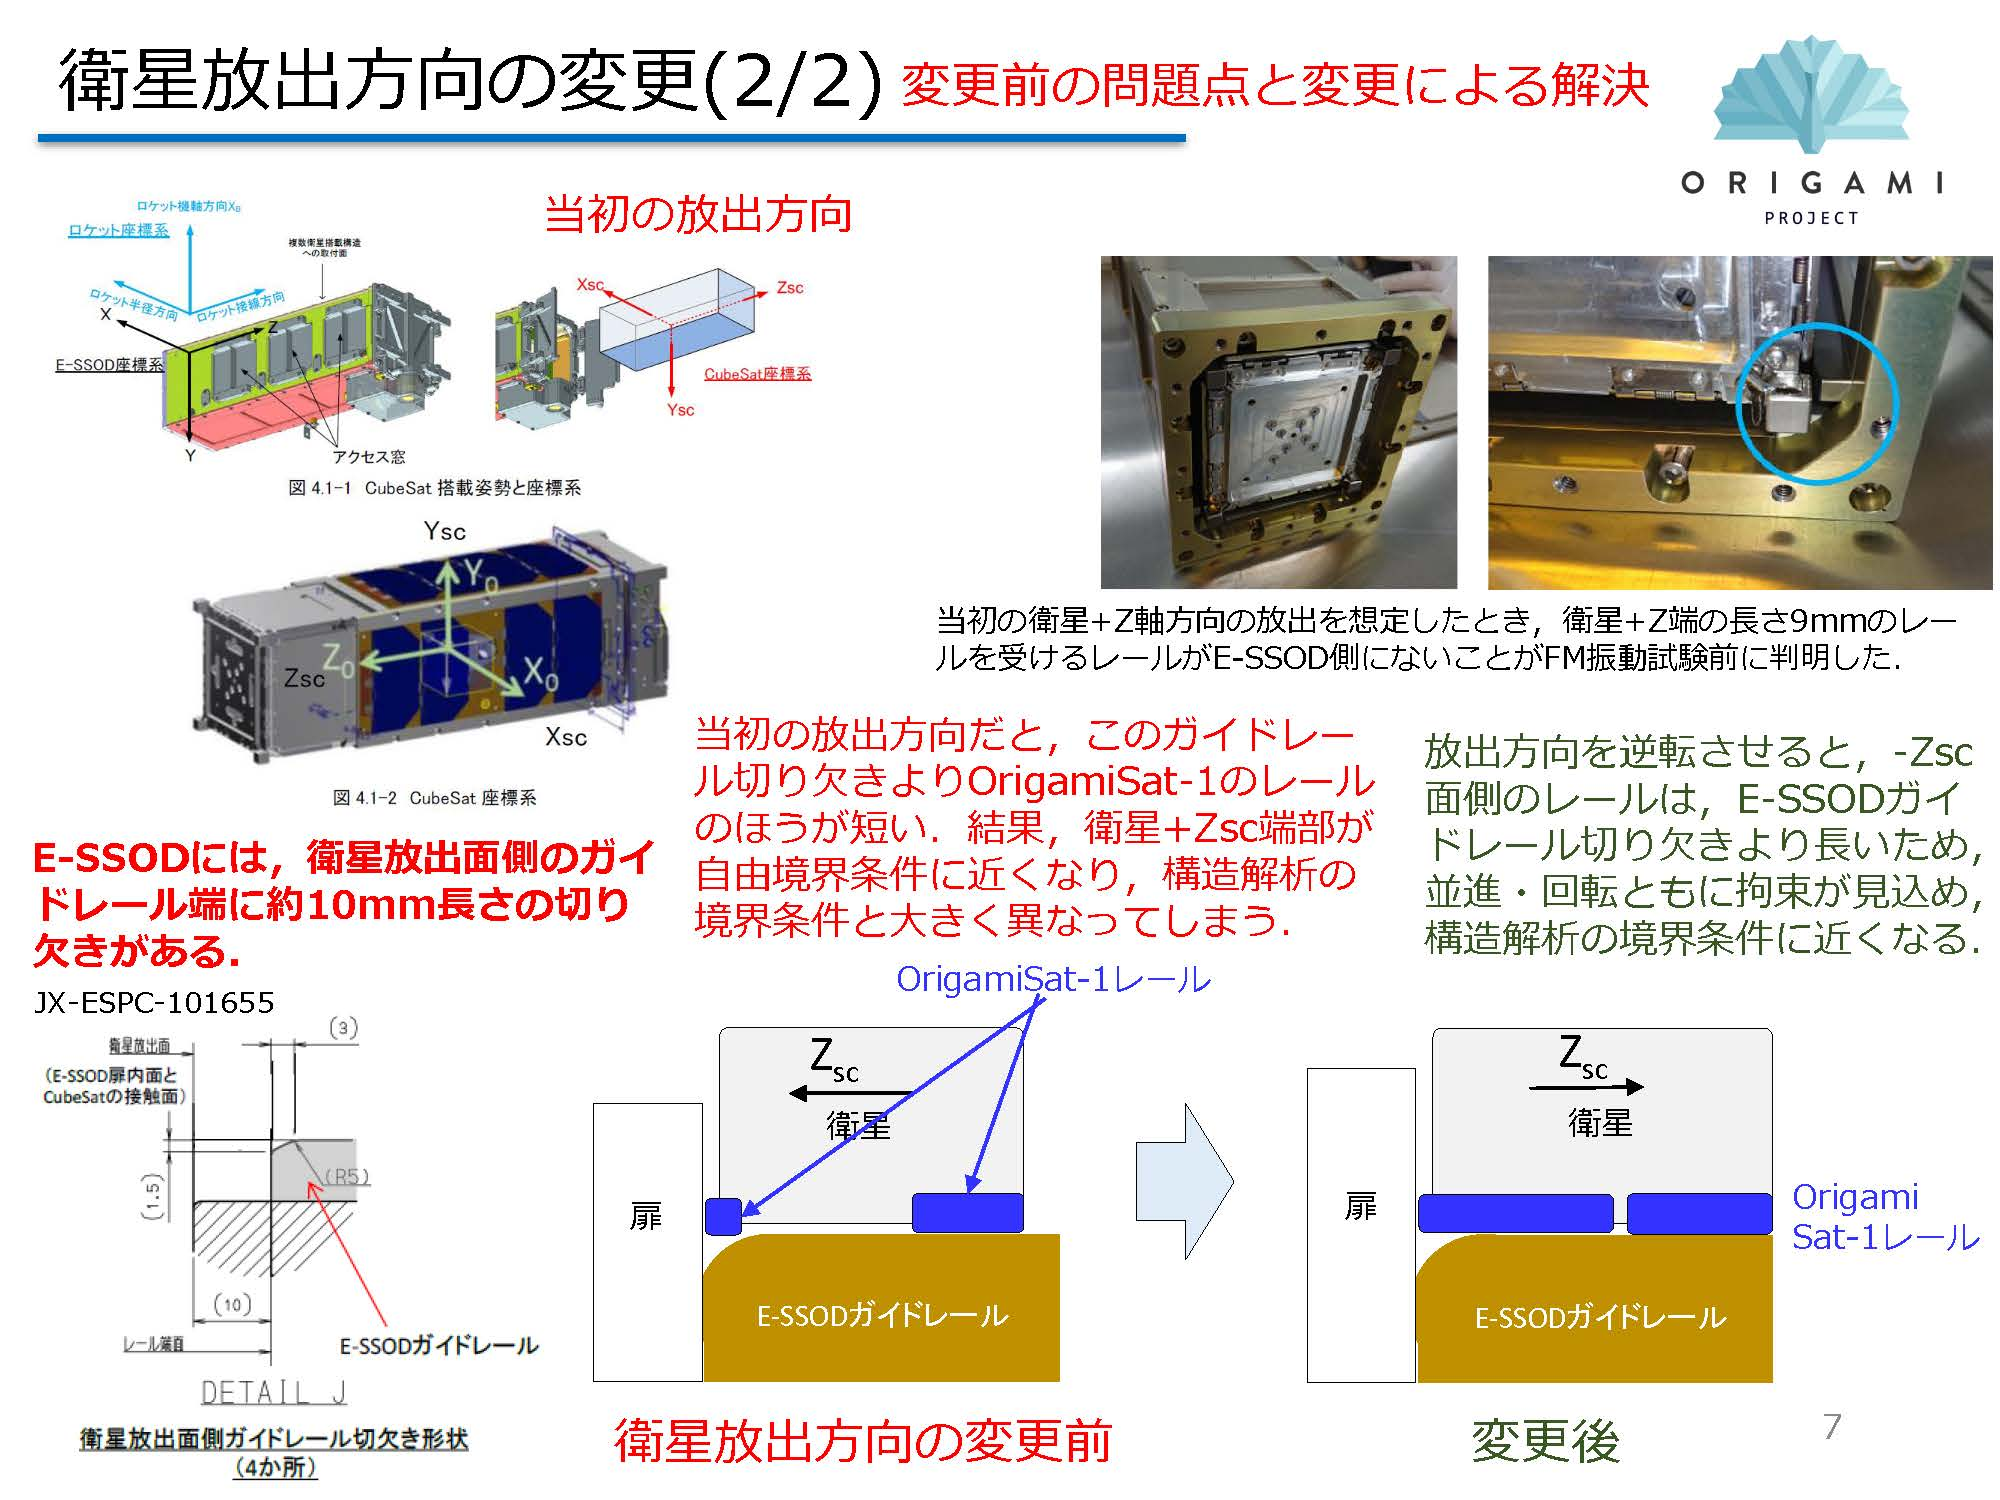
\includegraphics[width=10cm]{./06/fig/6-1_rail_trouble_2-2.jpg}
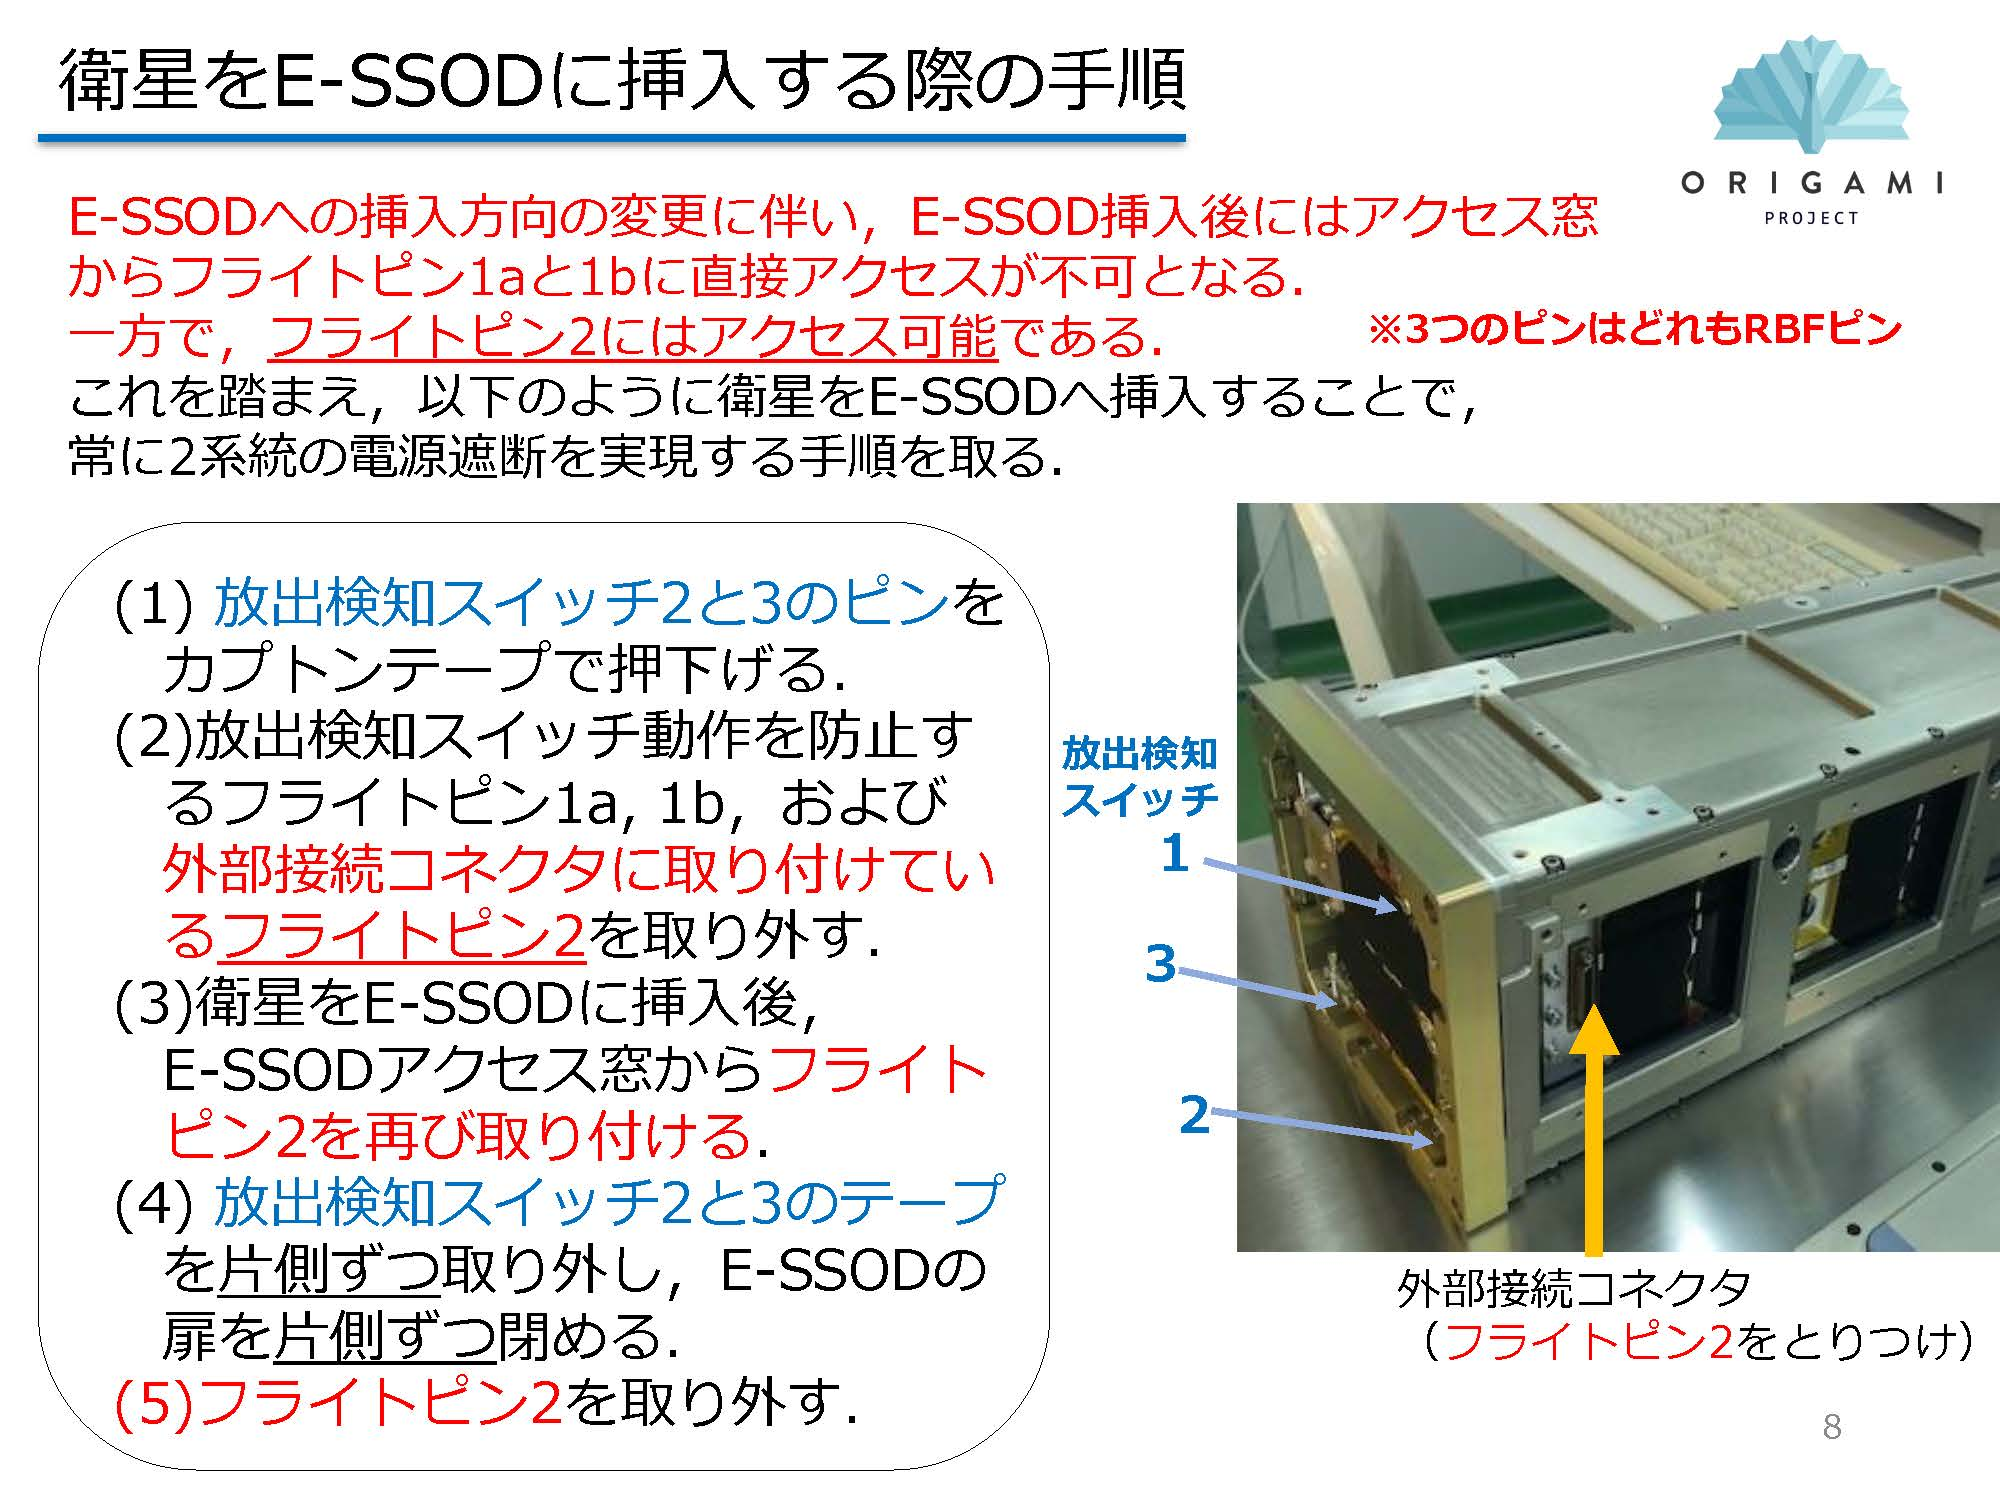
\includegraphics[width=10cm]{./06/fig/6-1_rail_trouble_2-3.jpg}
	\caption{レールの切り欠きに関する問題と対処 (OP-S1-0049
          OrigamiSat-1 衛星概要説明書より抜粋)}
	\label{6_1_trouble2}
\end{figure}

\subsection{磁力の逸脱}
本衛星は,姿勢制御に永久磁石を用いており,その磁気の目標値がICDで規定
されているが,FM組立後に磁力を計測したところ6面中3面 (磁力の弱い面) の
磁力がこれを逸脱した (磁力が大きくなる面についてはいずれも目標値内だっ
た).これは元々の目標値が本衛星のBBMの構体と磁石のみ
を用いた計測結果をロケット側に照会する形で決定されたものであり,FMのコ
ンフィグレーションと異なったことが原因であった.

対応としては,FMでの実績値について再度ロケットに照会し問題ないことを確
認していただきICDの目標値を規定し直す(改訂前:衛星各面に目標値を設定,改
  訂後:目標値は全面共通で最大磁力方向の値とし,これ以下であれば適合)ことで適合となった.

BBMの計測結果を提出するに当たり,逸脱する可能性を十分に考慮しマージン
を取った値も提示し,ロケット側の了解を取っておくことが重要であった.


